\documentclass[border=0pt,tikz]{standalone}
% Nature Portfolio / Scientific Data shared TikZ style for IRexp figures.
% Width: 183 mm double-column. Typography: Helvetica-class (phv).
\RequirePackage{tikz}
\RequirePackage{pgfplots}
\RequirePackage{xcolor}
\RequirePackage{helvet}
\IfFileExists{sansmathfonts.sty}{\RequirePackage{sansmathfonts}}{}
\renewcommand{\familydefault}{\sfdefault}
\pgfplotsset{compat=1.18}
\usetikzlibrary{
  arrows.meta,calc,positioning,fit,shapes.geometric,shapes.misc,
  backgrounds,shadows.blur,patterns,decorations.pathreplacing
}

% ---- Paul Tol / NMRexp-matched palette ----
\definecolor{nmrBlue}{HTML}{4A7EBB}
\definecolor{nmrBlueDark}{HTML}{2E5F8F}
\definecolor{nmrBlueLight}{HTML}{A8C8E8}
\definecolor{nmrPeach}{HTML}{E8B48C}
\definecolor{nmrNavy}{HTML}{1B3D5C}
\definecolor{nmrRed}{HTML}{C44E52}
\definecolor{nmrGreen}{HTML}{3D8B5E}
\definecolor{nmrOrange}{HTML}{D97B32}
\definecolor{ink}{HTML}{1A1A1A}
\definecolor{muted}{HTML}{7A7F85}
\definecolor{note}{HTML}{5C636A}
\definecolor{faint}{HTML}{E8EAEC}
\definecolor{ghost}{HTML}{C5C9CD}
\definecolor{tintBlue}{HTML}{EEF3F8}
\definecolor{tintGreen}{HTML}{EAF4EE}

\newcommand{\NatureFont}{\fontfamily{phv}\selectfont}
\newcommand{\PanelLabel}[1]{%
  {\NatureFont\bfseries\fontsize{8}{9.6}\selectfont #1}%
}
\newcommand{\FigBody}{\NatureFont\fontsize{7}{8.4}\selectfont}
\newcommand{\FigSmall}{\NatureFont\fontsize{5.5}{6.6}\selectfont}
\newcommand{\FigAxis}{\NatureFont\fontsize{7}{8.4}\selectfont}

\tikzset{
  nature arrow/.style={
    -{Latex[length=1.6mm,width=1.3mm]},
    line width=0.55pt, ink
  },
  nature arrow grey/.style={
    -{Latex[length=1.6mm,width=1.3mm]},
    line width=0.5pt, note
  },
  stage card/.style={
    draw=nmrBlueDark, line width=0.7pt, rounded corners=2.2pt,
    fill=white, inner sep=3pt, align=center, font=\FigBody
  },
  stage header/.style={
    fill=nmrBlueDark, text=white, font=\FigBody\bfseries,
    rounded corners=2.2pt, inner sep=2.5pt, align=center
  },
  soft card/.style={
    draw=ghost, line width=0.55pt, rounded corners=2.2pt,
    fill=white, inner sep=3.5pt, align=left, font=\FigBody
  },
}

\pgfplotsset{
  nature axis/.style={
    tick label style={font=\FigSmall, /pgf/number format/assume math mode},
    label style={font=\FigAxis\bfseries},
    title style={font=\FigBody\bfseries, color=ink},
    axis line style={ink, line width=0.5pt},
    tick style={ink, line width=0.45pt},
    major grid style={faint, line width=0.35pt},
    axis x line=bottom,
    axis y line=left,
    enlarge x limits=false,
    clip=false,
  },
  nature hbar/.style={
    nature axis,
    xbar,
    bar width=7pt,
    y=data,
    nodes near coords,
    every node near coord/.append style={
      font=\FigSmall, ink, anchor=west, /pgf/number format/fixed,
      /pgf/number format/1000 sep={,}
    },
    xtick=\empty,
    axis x line=none,
    y axis line style={ink, line width=0.55pt},
    ytick style={draw=none},
    y tick label style={font=\FigBody, ink, anchor=east},
    grid=major x,
    xmin=0,
  },
}

\usepackage[T1]{fontenc}
\usepackage{textcomp}

\begin{document}
\NatureFont
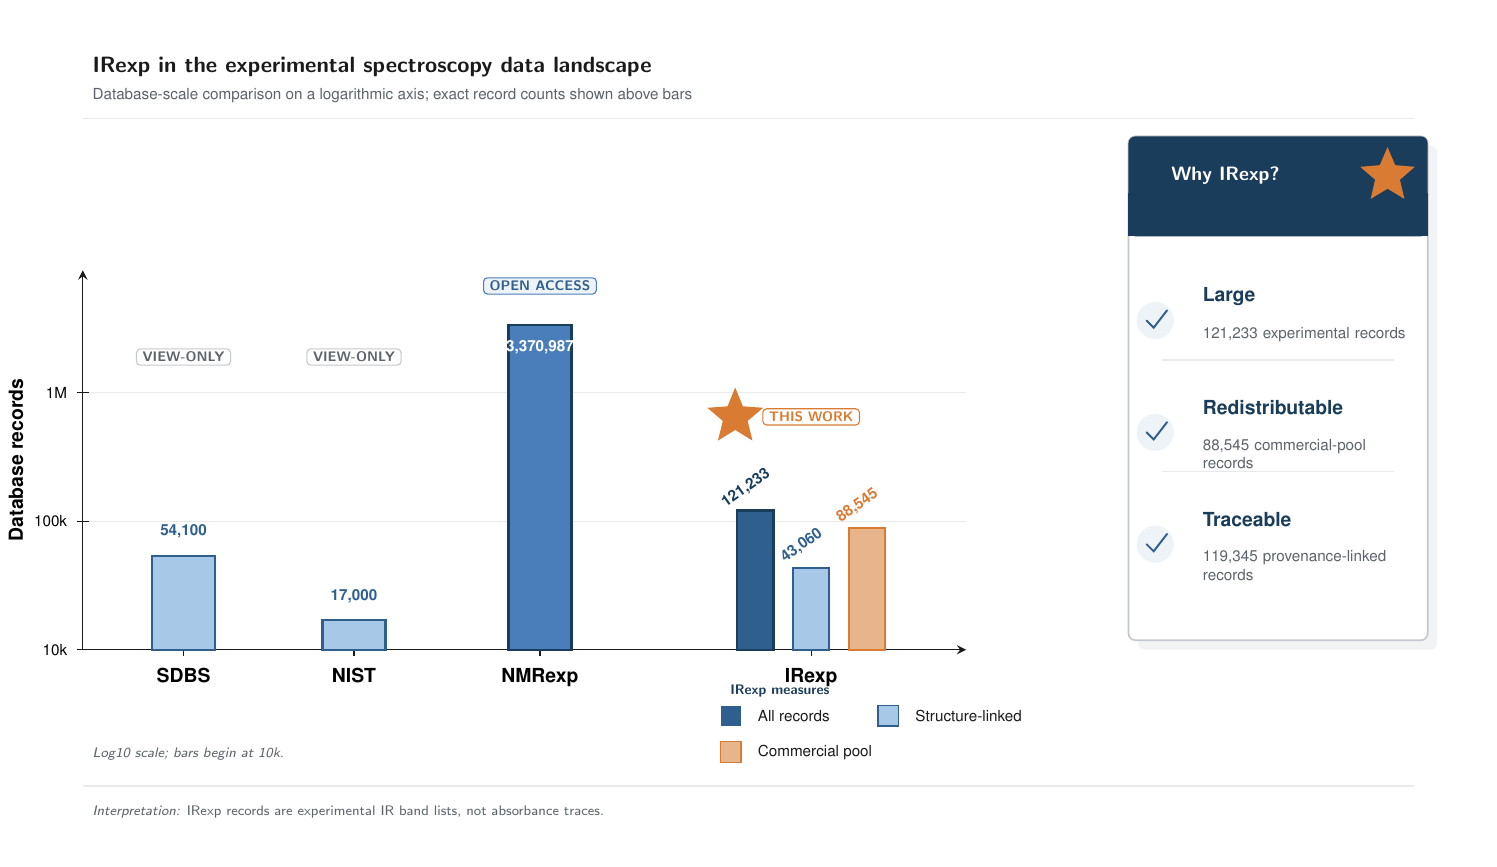
\begin{tikzpicture}[x=1mm,y=1mm]
  \path[use as bounding box] (0,0) rectangle (183,103);
  \fill[white] (0,0) rectangle (183,103);

  % Editorial header
  \node[anchor=west,font=\fontsize{8}{9.6}\selectfont\bfseries,text=ink]
    at (7,98) {IRexp in the experimental spectroscopy data landscape};
  \node[anchor=west,font=\FigSmall,text=note]
    at (7,94.3) {Database-scale comparison on a logarithmic axis; exact record counts shown above bars};
  \draw[faint,line width=.45pt] (7,91.5) -- (176,91.5);

  % Main log-scale comparison
  \begin{axis}[
    nature axis,
    at={(7mm,24mm)},
    anchor=south west,
    width=128mm,
    height=64mm,
    ymode=log,
    log basis y=10,
    log origin=infty,
    ymin=10000,
    ymax=9000000,
    xmin=.35,
    xmax=6.05,
    xtick={1,2.1,3.3,5.05},
    xticklabels={SDBS,NIST,NMRexp,IRexp},
    x tick label style={font=\FigBody\bfseries,align=center,yshift=-1pt},
    ytick={10000,100000,1000000},
    yticklabels={10k,100k,1M},
    ylabel={Database records},
    ylabel style={yshift=-1mm},
    ymajorgrids=true,
    axis x line*=bottom,
    axis y line*=left,
    clip=false,
  ]
    % Reference databases
    \addplot[ybar,bar width=8mm,draw=nmrBlueDark,fill=nmrBlueLight,line width=.75pt]
      coordinates {(1,54100) (2.1,17000)};
    \addplot[ybar,bar width=8mm,draw=nmrNavy,fill=nmrBlue,line width=.8pt]
      coordinates {(3.3,3370987)};

    % IRexp: grouped, deliberately not stacked because subsets overlap.
    \addplot[ybar,bar width=4.6mm,draw=nmrNavy,fill=nmrBlueDark,line width=.85pt]
      coordinates {(4.69,121233)};
    \addplot[ybar,bar width=4.6mm,draw=nmrBlueDark,fill=nmrBlueLight,line width=.85pt]
      coordinates {(5.05,43060)};
    \addplot[ybar,bar width=4.6mm,draw=nmrOrange,fill=nmrPeach,line width=.85pt]
      coordinates {(5.41,88545)};

    % Exact values
    \node[font=\FigSmall\bfseries,text=nmrBlueDark,anchor=south]
      at (axis cs:1,62000) {54,100};
    \node[font=\FigSmall\bfseries,text=nmrBlueDark,anchor=south]
      at (axis cs:2.1,19500) {17,000};
    \node[font=\FigSmall\bfseries,text=white,anchor=north]
      at (axis cs:3.3,3050000) {3,370,987};
    \node[font=\FigSmall\bfseries,text=nmrNavy,anchor=south,rotate=35]
      at (axis cs:4.69,143000) {121,233};
    \node[font=\FigSmall\bfseries,text=nmrBlueDark,anchor=south,rotate=35]
      at (axis cs:5.05,51000) {43,060};
    \node[font=\FigSmall\bfseries,text=nmrOrange,anchor=south,rotate=35]
      at (axis cs:5.41,104000) {88,545};

    % Access-status tags
    \node[rounded corners=1.4pt,draw=ghost,fill=white,inner xsep=2.2pt,inner ysep=1.2pt,
          font=\fontsize{5}{6}\selectfont\bfseries,text=note]
      at (axis cs:1,1900000) {VIEW-ONLY};
    \node[rounded corners=1.4pt,draw=ghost,fill=white,inner xsep=2.2pt,inner ysep=1.2pt,
          font=\fontsize{5}{6}\selectfont\bfseries,text=note]
      at (axis cs:2.1,1900000) {VIEW-ONLY};
    \node[rounded corners=1.4pt,draw=nmrBlue,fill=tintBlue,inner xsep=2.2pt,inner ysep=1.2pt,
          font=\fontsize{5}{6}\selectfont\bfseries,text=nmrBlueDark]
      at (axis cs:3.3,6800000) {OPEN ACCESS};
    \node[rounded corners=1.4pt,draw=nmrOrange,fill=white,inner xsep=2.2pt,inner ysep=1.2pt,
          font=\fontsize{5}{6}\selectfont\bfseries,text=nmrOrange]
      at (axis cs:5.05,650000) {THIS WORK};
    \node[star,star points=5,star point ratio=2.25,fill=nmrOrange,draw=none,
          minimum size=3.5mm] at (axis cs:4.56,650000) {};
  \end{axis}

  % IRexp grouped-bar key, aligned under the plot
  \node[anchor=west,font=\fontsize{5}{6}\selectfont\bfseries,text=nmrNavy]
    at (88,18.7) {IRexp measures};
  \fill[nmrBlueDark] (88,14.3) rectangle +(2.6,2.6);
  \node[anchor=west,font=\FigSmall,text=ink] at (91.5,15.6) {All records};
  \fill[nmrBlueLight,draw=nmrBlueDark,line width=.45pt] (108,14.3) rectangle +(2.6,2.6);
  \node[anchor=west,font=\FigSmall,text=ink] at (111.5,15.6) {Structure-linked};
  \fill[nmrPeach,draw=nmrOrange,line width=.45pt] (88,9.7) rectangle +(2.6,2.6);
  \node[anchor=west,font=\FigSmall,text=ink] at (91.5,11) {Commercial pool};
  \node[anchor=west,font=\fontsize{5}{6}\selectfont\itshape,text=note]
    at (7,10.8) {Log10 scale; bars begin at 10k.};

  % Sidebar callout
  \fill[ghost,opacity=.22,rounded corners=2.5pt] (141,24) rectangle (179,88);
  \fill[white,draw=ghost,line width=.6pt,rounded corners=2.5pt] (139.8,25.2) rectangle (177.8,89.2);
  \fill[nmrNavy,rounded corners=2.5pt] (139.8,76.5) rectangle (177.8,89.2);
  \fill[nmrNavy] (139.8,76.5) rectangle (177.8,82);
  \node[anchor=west,font=\fontsize{7}{8.4}\selectfont\bfseries,text=white]
    at (144,84.2) {Why IRexp?};
  \node[star,star points=5,star point ratio=2.2,fill=nmrOrange,draw=none,
        minimum size=4.2mm] at (172.7,84.2) {};

  \foreach \yy/\title/\desc in {
    68.9/Large/{121,233 experimental records},
    54.7/Redistributable/{88,545 commercial-pool records},
    40.5/Traceable/{119,345 provenance-linked records}
  }{
    \fill[tintBlue] (143.2,\yy-3.1) circle (2.35);
    \draw[nmrBlueDark,line width=.7pt,line cap=round]
      (142.1,\yy-3.1) -- (143,\yy-4) -- (144.7,\yy-1.8);
    \node[anchor=west,font=\FigBody\bfseries,text=nmrNavy] at (148,\yy) {\title};
    \node[anchor=north west,text width=26mm,align=left,font=\FigSmall,text=note]
      at (148,\yy-2.7) {\desc};
  }
  \draw[faint,line width=.4pt] (144,60.8) -- (173.5,60.8);
  \draw[faint,line width=.4pt] (144,46.6) -- (173.5,46.6);

  % Data-honesty footer
  \draw[faint,line width=.45pt] (7,6.7) -- (176,6.7);
  \node[anchor=west,font=\fontsize{5.2}{6.2}\selectfont,text=note]
    at (7,3.4) {\textit{Interpretation:} IRexp records are experimental IR band lists, not absorbance traces.};
\end{tikzpicture}
\end{document}
